%

% 2018 7. Разработка ядра логического вывода конфигураций каркасов функциональных блоков информационной системы по комплексной модели MDA.
% 2019 7. Разработка технологий и инструментальных средств создания размеченных документов на основе интерпретации комплексной платформонезависимой модели информационной системы.
% 2020 7. Разработка специализированного интерпретатора платформонезависимой модели, ориентированного на поддержку современных средств разработки интернет-приложений, функционирующих в среде Linked Open Data.

\documentclass[conference]{IEEEtran}
\IEEEoverridecommandlockouts
% The preceding line is only needed to identify funding in the first footnote. If that is unneeded, please comment it out.
\usepackage{cite}
\usepackage{amsmath,amssymb,amsfonts}
\usepackage{algorithmic}
\usepackage{graphicx}
\usepackage{textcomp}
\usepackage{xcolor}
\def\BibTeX{{\rm B\kern-.05em{\sc i\kern-.025em b}\kern-.08em
    T\kern-.1667em\lower.7ex\hbox{E}\kern-.125emX}}
%\usepackage[T1]{fontenc}
%\usepackage[utf8]{inputenc}
\usepackage{luatextra}
\usepackage{currvita}
\usepackage{minted}
%\usepackage{ulem}
%\usepackage[]{geometry}
% \usepackage[a4paper,margin=2cm]{geometry}
\usepackage{multicol}
\usemintedstyle{bw}
\usepackage{enumitem}
%\usepackage{indentfirst}
\setminted{fontsize=\small}

\providecommand{\sout}[1]{}



% *** CITATION PACKAGES ***
%
%\renewcommand\cite[1]{[[#1]]}

\usepackage{hyperref}
\hypersetup{
    % bookmarks=true,         % show bookmarks bar?
    unicode=true,          % non-Latin characters in Acrobat’s bookmarks
    pdftoolbar=true,        % show Acrobat’s toolbar?
    pdfmenubar=true,        % show Acrobat’s menu?
    pdffitwindow=false,     % window fit to page when opened
    pdfstartview={FitH},    % fits the width of the page to the window
    %pdftitle={},    % title
    %pdfauthor={Author},     % author
    %pdfsubject={Subject},   % subject of the document
    %pdfcreator={Creator},   % creator of the document
    %pdfproducer={Producer}, % producer of the document
    %pdfkeywords={keyword1, key2, key3}, % list of keywords
    %pdfnewwindow=true,      % links in new PDF window
    colorlinks=true,       % false: boxed links; true: colored links
    linkcolor=black,          % color of internal links (change box color with linkbordercolor)
    citecolor=black,        % color of links to bibliography
    filecolor=black,      % color of file links
    urlcolor=black,           % color of external links
    final=true
  }

\setmainfont{Times New Roman}

\begin{document}
\title{Representation of MDA Transformation with Logical Objects}

% \titlerunning{Implementation of a QMS with MDA}

\author{
\IEEEauthorblockN{Evgeny Cherkashin, Alexey Shigarov, Viacheslav Paramonov}
\IEEEauthorblockA{\textit{Matrosov Institute for System Dynamics and Control Theory of SB RAS,} \\
 \textit{Irkutsk Scientific Center of SB RAS} \\ 134 Lermontov Street, Irkutsk, 664033, Russia\\\{eugeneai,shig,slv\}@icc.ru}
}

% \tocauthor{Evgeny Cherkashin, Alexey Shigarov, Viacheslav Paramonov, Ljubica Kazi}

% \authorrunning{Evgeny Cherkashin, Alexey Shigarov \emph{et al.}}

% \email{\{eugeneai,shig,slv\}@icc.ru, ljubica.kazi@gmail.com}}

\maketitle

\begin{abstract} % 70-150 words
  The problem of software modeling having various models as sources and its transformation based on logical inference is considered.  Source models are converted into graphs of RDF and then processed with knowledge based system organized in a network of objects.  Various notation can be used to represent models, such as UML, SysML, CMMN, BPMN2.0, as well as RDF graphs and analyzed source code, having implemented a corresponding converter.  The objects are represented in the LogTalk programming language.  Objects query graphs and other objects implementing a scenario of a software system synthesis within Model Driven Architecture paradigm.

  Usage of such kind of transformation approach allows us to develop software system carcasses on the level of abstract models, involve various sources of model data in the transformation, define and structuring conversion knowledge as objects.  An example of a dataflow environment synthesis encapsulating Mothur library for new generation sequencing is presented.
\end{abstract}

\begin{IEEEkeywords}
model driven architecture, logical inference, resource description framework, LogTalk
\end{IEEEkeywords}

\section{Introduction}
\label{sec:intro}

% The simplest approach to a system improvement consists of the repetitive execution of the following steps over a level of organization under reingeneering:
% \begin{enumerate}
% \item imaging the target state of the system (future),
% \item comparison with the present state,
% \item assessment of the deviations from the target state,
% \item planning set of actions for reaching the target state,
% \item performing the planned set of actions,
% \item control of the achieving the target state by, e.g., checking the set of target criteria.
% \end{enumerate}

% Business process (BP) reingeneering usually starts from a technical audit (TA), the process of a system analysis of an organization structure, its problems and resources \cite{techaudit}.  The result of the TA is set of text documents describing the present state of the organization and its BPs on the various levels (social, administrative, technical, and physical).  The set comprises specifications of organization structure, BP models (AS-IS, TO-BE), target state requirements and restrictions, etc.

% [[Specification structure]]

% [[[Point of views: people resources, marketing, technology, IT, finance]]]

% [[Gathering information]]

% There are three general creative roles of stakeholders involved in the improvement and revealed during TA: \emph{problem owner}, \emph{knowledge owner}, and \emph{problem solver}.  Problem owner is the agent (person), who recognizes the problems in the current state.  This role describes future target state as a ranged list of \emph{requirements} and \emph{restrictions}.  Knowledge owner describes the states in technical terms of the problem domain.  The description contains structure of BPs, their sequences, parameters, causal relationship, control processes, etc.  Problem solver searches and devices a problem solution, relying on a problem solving methodology, respecting interests of the problem owner, and information acquired from knowledge owner.

% [[[How we can represent specifications as IT SUBSYSTEM of an existing system? dring the process of improvement]]]

% [[[Application of the nowadays modeling notations in specifications for the low levels]]]
% .....MOD to be improved with more expressive but complex notions of SysML (System Markup Language), BPMN--2.0 (Business Process Modeling Notation) and CMMN (Case Management Modeling Notation).  SysML used to describe organizational and administrative structures in higher degree of abstraction with respect to UML2, which is used at administrative and technical levels, and in the same time to be more detailed.  The usage of these modeling notation will allow to describe the present organizational structure more formally and precisely as a Computational Independent Model (CIM) and Platform Independent Model (PSM) of MDA paradigm, resulting the bridge between specifications and IT resource under development.

% Heaving described BPs structure and flows of an organization in the formal detailed multilevel form in SysML, we could construct an environment of a permanent IS research and development.  At the first stage, a most simple case is being realized: the description could be converted into check lists controlling conditions of business process starting and ending points. The second stage of implementation is the automation of planning after reaching a checked condition.  The third stage is to organize data processing according to the synthesized plan.  In the long run a refined specification description is being integrated with already used software.  All the stages are accompanied with a lot of useful information to be accumulated, forming the quality measurement, knowledge and analysis basis \cite{aiowa}.

% TOO MANY GOALS AND TOO COMPLEX SOFTWARE - SHOULD BE PRESENTED AS A COMPONENT DIAGRAM WHICH CAPTURES THE IDEA AND SERVES AS A BASIS FOR THE LONG-TERM DEVELOPMENT.THE IDEA WRITTEN THIS WAY IS TOO WIDE AND MISTY.

One of the main challenge of informational systems (IS), as well as other industrial software design, development is complexity expressed in its structure, integration with other software, fast prototyping on the stage of design.  Rising the stage of code generation of IS within the development to abstract level of design allows us to produce IS prototypes as early as the specification are formalized.  CASE--systems are usually developed close to standard industrial technologies; it is not popular in developing IS for small organization and startups, which is characterized with uncertainties of requirements and specification.

In order to support IS subsystems generation, we are to develop an expressive means for transformation from set of formalized models represented in UML, SysML, BPMN and other ones constructed with corresponding design tools.  The process of tradition programming should allow us to develop specialized versions for peculiar software design approaches, with conserving common practices as libraries.  One of the paradigm of the implementation could be object--orientation, which in context of knowledge based systems will allow us to have a powerful tools enabling knowledge structuring, manipulation, and encapsulation as transformation components.  % This technique should improve generative approaches is due to absence of transformation implementation techniques ``consuming and adapting previous experience'' expressed in transformational libraries, which are also absent.

The most investigated transformational approach of code generation, that goes beyond the CASE, is Model Driven Architecture (MDA).  MDA represents code generation as multistage process of model transformation.  The source code and initial data are produced from a Platform Specific Model (PSM) that represents IS implementation on a specific program and hardware platform.  PSM is obtained from a Platform Independent Model (PIM), which describe IS more abstract without platform specifics.  A part of PIM could be resulted from a Computational Independent Model representing the IS and its environment on conceptual, organizational, system level, which does not define information conversion (e.g., computation).

%Input models are stored in various format, including proprietary ones; they could be converted to OMG standard XMI representation.  XMI is a set of identified structural components,
CIM and PIM usually defined as a sets of SysML, CMMN, UML and other visual models, which saved in a standard way as XMI\footnote{XML Metadata Interchange} files.  Dispute these notations additional data for transformation can be obtained from Semantic Web (SW), for example, ontology definitions, literal names of entities in various natural languages, current state of processes, and so on.  The popular ways of model transformation, like ATL\footnote{ATLAS Transformation Language}, are based on transformation one XMI model to another XMI, and then to the code.  Involving SW data is problematic.

We propose a more general approach, where for all model sources a converter to RDF\footnote{Resource Description Framework} format, the standard SW data and knowledge representation, and the transformation is defined as object-oriented logical program in the LogTalk language.  This allows us represent the transformation as a scenario of objects exchanging messages, querying a SW graph fact database on model structures and SW data.  Object programming enables us to structure, manipulate the knowledge base with encapsulation, inheritance, extending and composition.

The \emph{object} of the research is the development of a technology for transformation implementation as knowledge based system and be capable to process heterogeneous model sources as a complex of CIM and PIM. The \emph{subject} of the paper is to describe above proposed data representation and transformation techniques.

\section{Architecture of MDA tools}

% (here we speak about how to convert BPMN, SysML and CMMN models into carcass of an Inform. System... various stages of processing, including input....)

The architecture of the transformation tools is based on the provision of uniformity of the transformation rules language and predicate input data representation.  That's why we require either to store all the input model data in SW graphs of ontologies, or provide an interface representing the source model as the ontology graph.  The ontologies could be served as RDF--files of triples or with servers having SPARQL endpoints.  A general architecture of the development tools is presented in Fig.~\ref{fig:archi}.

\begin{figure}[htb]
  \centering
   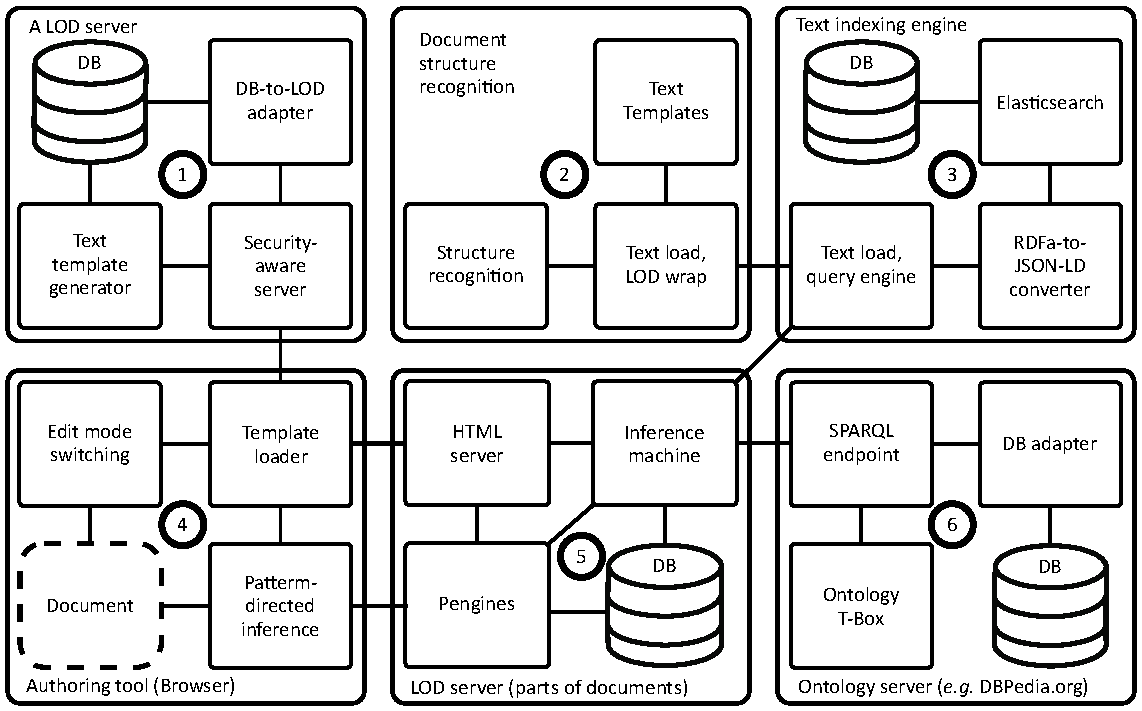
\includegraphics[width=1\linewidth]{pics/architecture-mda-lod-ext.pdf}
  \caption{Architecture of MDA transformational tools}
  \label{fig:archi}
\end{figure}

The MDA tools consists of the following main components:
\begin{itemize}
\item source model server (2), which stores and retrieve model data as RDF triples;
\item MDA transformation engine (1), which queries data from the server other SPARQL compliant servers (4);
\item the CIM (3) and PIM (6) model data sources;
\item indexing engine (5), which provides persistent utility means for text data storage and text processing interfaces.
\end{itemize}

All components interact by means of network protocols and use utf-8 encoded HTML, TXT, XML and JSON formats for data representation, which are expressive enough and easily debugged.  Inference engines also support SPARQL protocol for issuing subqueries.

The kernel of the system is MDA tool, which is a set of transformational modules (T--modules). Each T--module in a general case is a parameterized LogTalk object.  The object queries the Server of domain models, which is built on the base of ClioPatria \cite{Clio}, other objects and other Ontology servers for structural patterns.  These patterns are analyzed and the results are stored as the objects states, \emph{e.g.}, cashed in the indexing engine.  The states of the object represent PSM, which is translated into source code and initial data.

Input structures of CIM and PIM models are converted into graphs with converter adapters.  For example in Fig.~\ref{fig:archi} CIM (3) drawn in Modelio \cite{modelio} is converted to triples with a special module ``XMI to RDF converter''.  Similar converter is realized for PIM represented in UML.  This approach makes the input stage modular, and, consequently, easier extensible with new model types.

%IF WE EMPHASIZE SYSML, HOW IS IT RELATED TO SEMANTIC WEB TRIPLETS? THIS SHOULD BE EXPLAINED.

One of auxiliary RDF--compliant data sources is \texttt{DBPedia.org} containing naming literals in various languages, as well as relations, of the entities represented in Wikipedia.  This information can be used to describe user interface properties of the program objects, and referred by URI's from devised models.  For example, we can use DBPedia for constructing \texttt{title} and \texttt{placeholder} attributes of a web input widget, together with its label name text in user's locale and a help description.

% Some UML-structures (OCL) and relations may be interpreted constructively as methods of objects: events, handlers, subscribers, database triggers and selectors (lookups widgets).

\section{RDF representation of the models}
\label{sec:rdf-repr}

The past 20 years of unhurried SW technologies development formed descriptions of commonly used domains and represented them as W3C approved ontologies.  It enables system designer and programmer to use globally identified resource references (URI), and ontology representation standards (RDF, RDFa, TTL, etc.), which are implemented in various programming environments as libraries.  This results in a globally approved in various software projects knowledge and data base, the common foundation of a domain description.  This is why, we decided to represent the source model data in the SW framework too, enriching the existing knowledge with a specific domains.  From other hand side, converting the complex tree-like structures used for model representation to set of triples, \emph{i.e.}, facts for inference machine, enables us to use Prolog--based engines for transformation definition.

In order to meet SW requirements, each model should be identified with a global URI, and in addition, its prefix could be defined.  All relations and attributes must be expressed in a SW ontology, which should preferably be a standard one and have a publicly accessible formal definition.  The entity names and their relation expressed with the source notation must be convertible to the RDF definition upon request from transformation engine.

\subsection{Entity denotation}
\label{sec:ent-def}

Entity identification and naming in RDF have various aspects.  An entity or a relation exist if they are defined or referred with its URI.  An entity can be named by means of a relation with its URI, \emph{e.g.}, \texttt{dc:title} or \texttt{rdfs:label}.  The relation refers to a \texttt{literal} string with a corresponding name in a natural language (defined by an attribute).  Each model structure element or a relation in a model notation must have a corresponding notation in an model representation ontology.

As the entities have global identification, their mentioning in different models denote the same object, \emph{e.g.}, in a BPMN diagram, a record object could be created of a type defined in an UML Class Diagram.  The references of an entity of a model from another model can be done as RDF names of a form \texttt{<prefix>:<identifier>}, where \texttt{<prefix>} is the prefix of the model, where \texttt{<identifier>} is defined.  Most UML and other modeling software do not restrict names of the identifiers, together with their semantics, which is defined with transformation tools.

%[[ What else it is necessary to describe here?]]

\subsection{Model extensions}
\label{sec:mod-ext}

A flexible modeling tools also allow designer to extend a notation of a model (metamodel).  For example, all UML diagrams support \emph{stereotypes}, \emph{tag values}, and \emph{object constrains}.  Stereotypes declare an extended set of properties for an object or relation, \emph{e.g.}, in UML Class Diagram stereotypes are used to define the kind of a class.  If a class is assigned standard \texttt{<<interface>>} stereotype then it is an interface definition.  By default all classes are standard \texttt{<<class>>}-es.  The same is used to describe relations between use cases in Use Case diagram.  A use case can \texttt{<<include>>} another one or be \texttt{<<extend>>}-ed with another use case.  User-defined stereotypes can express various aspects of classes, \emph{e.g.}, we can define the storage class as an ORM\footnote{Object Relation Mapping} for a class by \texttt{<<RDBMSRecord>>} stereotype.  In this case, class is added to set of classes describing a relation database records, all relations between such classes are interpreted as rational (one--to--one, one--to--many, many--to--many, mandatory, etc.) relations.  One entity can be assigned many stereotypes.

Tag values allow one to associate a string value identified by a string key, which are somehow interpreted with a transformation procedure.  For example, the easy way of providing of an interface label name for an object \texttt{age} field in a class defined in a Class Diagram is an association the field with tag name \texttt{interface-label-name} as ``\texttt{Age}'' string.  Using RDF, we can change the tag name to \texttt{dc:title} and value can be interpreted as URI, \emph{e.g.}, to a \texttt{DBPedia} object.

The usage experience of stereotypes and tag values resulted in recognition of the fact, that assigning a stereotype usually implies definition of a set of regular tag values.  UML standard of version 2.4 fixed this observation, allowing formal definition the set of tag values for user-defined stereotypes.  Special user interfaces were developed to control assignment a stereotype to an entity.  As stereotype does not provide a value in its association, table name for \texttt{<<RDBMSRecord>>} an optional tag value can be defined for this purpose, \emph{e.g.}, \texttt{rdbms:table-name}.  UML-2.4 explicit stereotype descriptions is a powerful tool for attributing entities with additional information.

% [[[Resume of some kind]]]

\subsection{Other sources of model data}
\label{sec:other-models}

When implementing complex software, which are composed from existing subsystems, their specifications can be additional sources of model data.  For example, in our project \cite{bit2019}, the main PIM model is extracted from source code of the original library Mothur and converted to TTL (turtle) representation.  This approach requires one-time programming for adaptation of the sources, but for each new version of the library we can obtain new version of the PSM without additional analysis.  %Formal rules of the source code analysis ad interpretation as PSM can also assist in finding errors in the source code.

% [[PSM libraries....???]]


\section{Related works}

The most widely used technology of model transformation is ATL (ATLAS Transformation Language) \cite{atl} and its predecessor QVT, an OMG standard \cite{QVT}.  The language and its engine supports conversion from one XMI model to another one in the same XMI format.  The language structures describe recognition of properties of compositions of the source model and direct construction of new structures in the target model.

Similar to ATL, Transformation Model Representation Language (TMRL) is developed in \cite{nikita} but oriented on visual representation of a knowledge base with following conversion in various production rules in CLIPS and OWL.  The visual presentation of transforming rules are used also in \cite{GT}.  In \cite{azis}, ATL is used to transform Computational Independent Model (CIM) represented as BPMN diagram into set of UML diagrams, defining PIM. Paper \cite{Rhazali} proposes a model transformation CIM to PIM for web-applications, where CIM is represented with State and Use case UML-Diagrams logically connected with ATL rules.  In \cite{Hamid} is proposed an evaluation of security aspects of distributed applications using MDA description; the evaluation is implemented a logical inference over the MDA synthesized logical security models. The paper \cite{Zdun} is considered a highly decoupled distributed event-driven application environment, whose design and functioning is dynamically controlled by its three-level DSL\footnote{Domain Specific Language} description and MDA transformations, which support change propagation.

%Paper \cite{Malki} presents a practical approach with four-level ATL-description from HTML-page to a LOD structure (via stage of an MDA PIM). In \cite{uml2owl}, a converter of UML package structures represented in XMI was developed as a XSLT transformation. A wide overview of Western approaches to program transformation is given in \cite{Dama}, a transformation language PROMOL is suggested as well as its logical semantics. OMG proposed ODM standard \cite{odmprof} for knowledge modeling.  A Visual Ontology Modeler \cite{odnext} is being developed for building and verifying OWL ontologies for ODM~1.0, as well as in the reverse direction, ontologies are represented as UML Class Diagrams \cite{odmvis}.

% An XML based specifications are used in representing metadata about web services, WSDL \cite{wsdl}, and the WS-BPEL language \cite{wsbpel} for describing orchestration of web services within execution of an instance of a business process.  The idea of the language is to describe complex systems down to Web Services units, their internal and external structure and behavior, as well as services interaction in the script instance.

Thus, the majority of the presented techniques are closed with respect of XMI file format: the source data and the result of the transaction are represented in it, and it goes beyond only on the stage of the source code generation.  Our approach allows one to use other sources (not being presented in XMI) of model information, as well as general purpose libraries in implementation of the transformation engine.  Usage of object-oriented logical language LogTalk allows us powerfully structuring and manipulate knowledge base. % by means of the object encapsulation, inheritance, and composition.

% \subsection{Ontology Usage in Model Representation}
% \label{sec:use-onto}

% SysML is the dedicated system-level UML-based notation proposed by the OMG. In research \cite{raslan} system design productivity is addressed as one of the main challenges. Some suggested approaches are increasing the level of abstraction and automation, as well as producing executable specifications. In \cite{natale}, model driven development is used for the construction of complex embedded systems integrating software and firmware. A SysML system model is devised according to the platform-based design paradigm, in which a functional model of the system is paired to a model of the execution platform. Subsystems are refined as Simulink models or hand-coded in C++.

% The SysML standard is attracting more attention of hardware designers as UML and SysML have been used to automatically generate an HDL code written in SystemC, Verilog and VHDL. In \cite{boute}, contrarily to the existing works, authors propose the new reverse engineering approach to generate SysML definition of block and internal block diagrams from VHDL code. Code generation is done on the basis of a set of well-defined mapping rules between SysML and VHDL concepts.

% UML profiles like SysML and MARTE have been a major research topic in electronic system design, but are mainly applied for specification and analysis in early design phases.  Research \cite{mish} addresses the problem of the High-Level Synthesis (HLS), \emph{i.e.} physical implementation aspect of electronic systems, which need diversity of design models and levels of abstraction.  To overcome the conflict between a higher degree of abstraction and necessary details for further synthesis, modular interfaces are introduced as object-oriented synthesizable technique. In \cite{mish}, SysML is used as an adequate modeling language for modular interfaces and C/C++/SystemC-based HLS. Authors extended SysML with annotations for synthesizable SystemC and high-level synthesis constraints and implemented a code generation scheme to achieve design flow automation. They used SysML editor Artisan Studio with industrial case study to demonstrate the applicability of SysML as a front-end for HLS.

% In \cite{tom16} UML/SysML is used to model avionics.  The implementation language is C\# with using libXML for XMI import and processing.  Generated objects represent each syntactic element (\texttt{struct}, \texttt{enum}, function, \emph{etc.}), which represents the target source code.  Authors implemented only State Machine diagram transformation.

% % \cite{fab} % the lost reference

% Some experience of representing document flows are obtained by commercial software vendors developing Directum, Documentum systems automatizing Russian municipal institutions and state corporations.  Directum uses SysML state--like block diagrams to define flow of documents and the ISBL object-oriented language to express sophisticated behavior.

% % NOT ONLY THIS, THERE IS MORE NEEDED IN THE RELATED WORK SECTION: BUSINESS PROCESS MANAGEMENT SYSTEMS, BUSINESS RULES MANAGEMENT SYSTEMS, WORKFLOW MANAGEMENT SYSTEMS.

% In our research we focus on representation of ISO 9001 entities in SysML and other DSLs translatable to RDF, and the MDA transformation logical inference representable as LogTalk objects.

% \section{SysML representation of QMS}

% QMS is represented in SysML with nine diagrams \cite{sysmlpres}.  QMS requirements is represented with new (with respect to UML) \emph{Requirement Diagram}, describing stated structural and logical constraints. Structural aspects are represented with following UML2 diagrams:
% \begin{itemize}
% \item \emph{Block Definition Diagram} decomposes structure of activities, attributes and objects on elements;
% \item \emph{Internal Block Diagram} models interaction of the decomposed elements and their data flow; its descendant new \emph{Parametric Diagram} describes model of block attribute relationships;
% \item \emph{Package Diagram} organizes models in packages in various ways.
% \end{itemize}
% Behavioral aspect of a QMS is expressed with UML2
% \begin{itemize}
% \item \emph{Use Case Diagram}, which expresses functions of the system and their mutual relationships;
% \item \emph{State Machine Diagram} defines the states of the blocks and transitions between the states;
% \item \emph{Sequence Diagram} describes the order of messages between blocks and actors;
% \item \emph{Activity Diagram} represents computational process of converting data enclosed in blocks.
% \end{itemize}

% BPMN2.0 diagram is used to describe imperative procedures, it is very expressive diagram representing functions and involving agents, together with their relationships.  CMMN represents declarative aspects of the QMS especially data structures, processing stages, events and check points (milestones).  Adding BPMN2.0 and CMMN diagrams to SysML diagram set creates a redundancy, but in the same time it allows one to use more rich tool set for QMS modeling.

\section{Technique of Transformation Implementation}
\label{sec:tech-imp}

The main idea behind implementation of transformation engine is an usage of an object logical programming language meeting the following constraints:
\begin{itemize}
\item support multiple sources of model data,
\item first-order language for definition of the transformation,
\item transformation is represented as rules,
\item rules should be encapsulated in objects,
\item objects should query other objects for results,
\item means for transformation configuration and scenario description,
\item knowledge manipulation, including composition,
\item expression and query of RDF entities.
\end{itemize}

%The multiplicity of source data is archived with conversion of source structures to RDF triple sets, and object orientation of transformation representation: objects are encapsulations of model data.

SWI-Prolog with macro package LogTalk meet these constraints.  The LogTalk objects encapsulate Prolog first-order language rules as methods.  Each object is respected as a knowledge base of encapsulated rules.  Objects can be inherited (as prototypes or classes), parameterized, and composed with \emph{categories}.  In inheritance, methods can be reprogrammed implementing refined knowledge set.  Configurations are implemented as a prototyping hierarchies: in inheritance, a configuration are refined by replacing and adding new values.  Scenarios are implemented as an ordered sets of methods.  Finally, SWI-Prolog has a good LogTalk compatible RDF library strongly tied to the language itself.  The library represents RDF entities in a W3C compliant way.

% [[Rule representation in Prolog]]

% Existing popular approaches of implementing Platform independent model (PIM) to Platform specific model (PSM) transformation, taking into account the runtime and other implementation platform features.  The first approach is model-to-model transformation with a model transformation language, such as QVT-X, ATL, \emph{etc.}  In this case PIM and resulting PSM are represented as X MI files.  Model transformation language rules recognizes structures in PIM and construct structures of PSM, having account various \texttt{boolean} conditions calculated with helper rules. The second variant of transformation is realized with Domain Specific Language (DSL) infrastructure \cite{stratego}.  The transformation procedure is presented as translation of one DSL instance, \emph{i.e.} PIM, to an instance in another language.


%Resume
%Our approach is based on common known in AI tools, but requires additional programming of libraries of model transaction objects.

% \subsection{LogTalk as transformation engine}
% \label{sec:logtalk-engine}

% The direct way of a transformation implementation is to use \textsc{Prolog} or a functional language, and we use \textsc{Logtalk}, a macro package of Prolog.  The main advantage of the language usage is knowledge structuring thanks to its object-orientation.  Objects are used for representation of the source PIM model and the resulting PIM structures as well as source code generators.  Moreover, the transformation rules are easily integrated with libraries processing LOD and LOD warehouses.


\subsection{SWI-Prolog Semantic Web Library}
\label{sec:swi-sw}

SWI Prolog standard distribution contains library for RDF processing.  The library represents URI as a corresponding functor with atom argument. This structure can be constructed with a special form \texttt{<namespace>:<identifier>}.  Library contains predicates for loading graphs from files and internet sites, store them in various text based and binary formats for later use.

The library support queries for the graphs as a predicate query and as SPARQL.  There is a basic query optimization.  For the subclass and subpropery relation, library realizes transitive closure, which can be used in the predicate queries.  The library imported in LogTalk as an object, that is an encapsulation of all the library predicates.

% \subsection{Semantic Server ClioPatria}
% \label{sec:clio-descr}
% [[ClioPatria]]
\subsection{LogTalk Methods}
\label{sec:lgt-methods}

LogTalk object consists of only encapsulated predicates (methods), some of them can be defined as dynamic, implementing object state.  LogTalk as a macro package provides two kind of objects: static and dynamic.  Static objects is defined and instantiated during compilation, dynamic ones are created with \texttt{create\_object/4} usually at runtime.  Static parameterized objects can be considered as third way of instantiation.  The role of an object is defined with relation to other objects, \emph{e.g.}, instances of a class are the objects, which are \verb|instantiates/1| its class.

Static object instances are used for defining configurations, scenarios, interfaces to input and output targets (streams, models), graph databases, and other global compile time known entities.  Their main role is structuring Prolog rule set.  Dynamic objects are used in construction of PSM objects, currently, each instantiation is an entity of target programming language.  Parametrized objects are facade interfaces to other objects (contexts), \emph{e.g.}, input targets and graph databases.  These objects enables programmer to define recognition rules over set of structures provided it with parameters.  Parameterized objects should be stateless, in this case, LogTalk compiles it in statically executed code.

%%%%% Methods can be redefined during inheritance.  Sending to the redefined method is done with ``\texttt{\^\^}'' message to self.

% [[Idea how to implement objects, methods, instantiations, references, calls]]

\subsection{PSM Representation}
\label{sec:blocks}

PSM and source code generation are represented with \texttt{code\_block} objects. The idea was taken from \verb|llvmlite| library.  The code block object have the following interface:
\begin{minted}{logtalk}
:- protocol(code_block_proto).
:- public([
   append/1, prepend/1,  % Manipulation of PSM
   clear/0,              % content as a list
   remove/1,             % of ordered items.
   item/1, items/1]).    % List the items.
:- protected([
   renderitem/2,  % Converting items to code lines.
   render_to/2]). % Storing lines to a stream.
:- end_protocol.
\end{minted}

The \verb|code_block|--objects consist of source code string lines, structures denoting source code, objects, and other code blocks. Each item is accessed via \verb|item/1|.  The type of the element is defined by outer functor of the argument, \emph{e.g.}, we define with \verb|append(attributes(L))| a list \verb|L| of attributes of a class.  The way of rendering the sources is implemented by subclassing the object and realizing \verb|render/1| and \verb|renderitem/2|.  The first argument of \verb|renderitem/2| is the \verb|item/1|--structure to be rendered, and the second one is the list of strings representing generated source code.  Elements of a code block can be \verb|append|ed, \verb|prepend|ed and \verb|remove|ed.  We specially disallow inserting \verb|item|s into code blocks, as it will make object and its database more complex.  Instead, programmer can add an \verb|item| being another code block, inserting its content in the outer block.

If needed the item's definition can include provision information which can be used in result construction, when its object being queried.

\subsection{Defining rules of transformation}
\label{sec:mda-rules}

Transformation process is organized as a scenario of connected transformational objects (in terms of LogTalk).  Scenario is programmed as a special object defining transformation by means of calling \verb|tr/N| rules.  Rules recognize structures in the input graph elements and constructs code blocks.

\begin{minted}{logtalk}
:- object(direct(_Package,_LocalProf,_CodeProf)).
:- public([tr/4,tr/3]).
:- protected([package/1, profiles/2, profile/1]).
package(Package):- parameter(1, Package).
profile(Profile):- parameter(2, Profile).
profile(Profile):- parameter(3, Profile).
profiles(L):-
    findall(Profile, ::profile(Profile), L).
tr(class, Class, ClassID):- ::package(Package),
    query(Package)::class(Name, ClassID),
    create_object(Class,  % inherits code_block
        [instantiates(class)],[],[]),
    create_object(Attributes,
        [instantiates(params)],[],[]),
    create_object(Methods,
        [instantiates(methodlist)],[],[]),
    Class::append(name(Name)),
    forall(
        ::tr(attribute,Attribute,ClassID,_AttrID),
        Attributes::append(Attribute) ),
    forall(
        ::tr(method, Method, ClassID, _MethodID),
        Methods::append(Method) ),
    Class::append(attributes(Attributes)),
    Class::append(methods(Methods)).
tr(attribute, Attribute, ClassID, AttributeID):-
    ::package(Package),
    query(Package)::attribute(Name,ClassID,AttrID),
    create_object(Attribute,
        [instantiates(param)],[],[]),
    Attribute::append(name(Name)).
tr(method, Method, ClassID, MethodID):-
    ::package(Package),
    query(Package)::method(Name,ClassID,MethodID),
    create_object(Method,
       [instantiates(method)],[],[]),
    Method::append(name(Name)).
:- end_object.
\end{minted}

The previous listing uses static parameterized object \verb|query/1|, whose context argument is a graph representing model under transformation.  This is a powerful LogTalk abstraction instrument, which reduces necessity of adapter object creation in dynamic memory.  The SPARQL queries are encapsulated in methods.

\begin{minted}{logtalk}
:- object(query(_XMI)).
:- protected(xmi/1).
:- public([class/2, attribute/3, method/3]).
xmi(XMI) :- parameter(1, XMI).
class(Name, ID):- ::xmi(XMI),
    XMI::rdf(ID,rdf:type,uml,'Class'),
    XMI::rdf(ID,rdfs:label, literal(Name)).
attribute(Name, ClassID, ID):-  ::xmi(XMI),
    XMI::graph(G),
    XMI::rdf(ClassID, G:ownedAttribute, ID),
    % XMI::rdf(ID, rdf:type, uml,'Property'),
    XMI::rdf(ID, rdfs:label, literal(Name)).
method(Name, ClassID, ID):- ::xmi(XMI),
    XMI::graph(G),
    XMI::rdf(ClassID, G:ownedOperation, ID),
    XMI::rdf(ID, rdfs:label, literal(Name)).
:- end_object.
\end{minted}

The following example shows rendering class for Python classes. It contains public methods for defining class elements.

\begin{minted}{logtalk}
:- object(class, specializes(code_block),
    imports([named])). % A category of named entities
:- public([classlist/1, methods/1, attributes/1]).
classlist(ClassList):- % List of base classes
    ::prepend(classlist(ClassList)).
attributes(Attributes):- % List of attributes
    ::prepend(attributes(Attributes)).
methods(MethodList):- % List of methods
    ::append(methods(MethodList)).

renderitem(Item, Result):- % Default
    ^^renderitem(Item, Result).
render(Result):- % Render the class
    ^^render(Name), % Call inherited method.
    ( ::item(classlist(List)) ->
      List::render(ClassList),
      root::iswritef(Signature,'class %w(%w):',
        [Name, ClassList]);
      root::iswritef(Signature,'class %w:',
        [Name]) ),
    root::indent, % Add an indent
    ( ::item(attributes(Attributes))->
      Attributes::render(DefAttrList),
      root::iswritef(ConstructorDef,
        'def __init__(self, %w):',
        [DefAttrList]),
      root::indent,  % more indent
      Attributes::items(InstanceAttrs),
      findall(S, ( % initialize attributes
         lists::member(Attr, InstanceAttrs),
         Attr::item(name(AttrName)),
         root::iswritef(S, "self.%w=%w",
           [AttrName, AttrName])
         ), AttrAssigns),
        root::unindent,
        AttrList=[ConstructorDef|AttrAssigns];
        root::iswritef(ConstructorDef,
          'def __init__(self): ', []),
        root::indent,
        root::iswritef(Pass,'pass', []),
        root::unindent,
        AttrList=[ConstructorDef, Pass] ),
    ( ::item(methods(Methods))-> % if any ...
      Methods::render(MethodList);
      MethodList=[] ),
    lists::append(AttrList,MethodList,StringList),
    root::unindent, Result=[Signature|StringList].
:- end_object.
\end{minted}

Let us do some remarks.  Class method \verb|root::iswritef/3| is used to generate source code with a tab indent organized by \verb|root::indent| and \verb|root::unindent| predicates.  List \verb|Result| of \verb|render/1| specially not flatten in order to not use \verb|append| operations.  The object imports category \verb|named|, which defines behavior for named instances.

% \subsection{Categories}
% \label{sec:cats-impl}

LogTalk \emph{categories} is very useful way of implementing a common functionality among a set of entities.  For example, programming language objects have an identifier and, optionally, type description.  These properties are implemented as two categories.
\texttt{named}, and its child \texttt{namedtyped}.
\begin{minted}{logtalk}
:- category(named).
:- public([name/1, render/1]).
:- protected([renderitem/2]).

name(Name):- ::prepend(name(Name)).

renderitem(name(Name), String):-!,
    atom_string(Name, String).

render(String):-
    ::item(name(Name)),
    ::renderitem(name(Name), String).

:-end_category.
\end{minted}

The category implies interface of \texttt{code\_object} for the object being enriched with it.  The second category definition as well as all the sources of transformation objects are stored at \texttt{github.com} \cite{ghsrc}.  % The second example adds type to the object.

% \begin{minted}{logtalk}
% :- category(namedtyped, extends(named)).
% :- public([type/1,render/2,separator_option/2,
%    list_separator/1]).
% :- protected([renderitem/2]).

% type(Type):-
%    ::append(type(Type)).

% renderitem(Item, String):-
%    ^^renderitem(Item, String),!.
% renderitem(type(Type),String):-!,
%    ::list_separator(Separator),
%    writef::swritef(String, '%w%w', [Separator, Type]).

% render(Middle, String):-
%    ^^render(SName),
%    (
%      ::item(type(Type)) ->
%      ::renderitem(type(Type), SType),
%      string_concat(SName, Middle, _1),
%      string_concat(_1, SType, String) ;
%      SName = String
%    ).

% render(String):-
%    ::render("", String).

% list_separator(Separator):-
%    ::separator_option(Name, Default),!,
%    root::option(Name, Separator, Default).

% :- end_category.
% \end{minted}

% Similarly lists .... [[(list of superclasses, variables,...)]]

%In the same way, we can construct procedures for creating structures of databases and populating them with initial data.

% SO, IT IS TRANSFORMATION OF BUSINESS PROCESS MODELS (GRAPHICALLY SET) INTO FORMAL LANGUAGE, SUITABLE FOR AUTOMATED REASONING? HOW IS IT COMBINED WITH DATA FROM THE DATABASE? HOW THE DATA FROM THE DOCUMENT MANAGEMENT SYSTEM IS EXTRACTED INTO DATA SUITABLE FOR AUTOMATED REASONING?

% THE POINT IS:
% 1. HAVING DOCUMENT MANAGEMENT COMBINED WITH THE BUSINESS PROCESS MODELS
% 2. COMBINING DATA FROM DOCUMENT MANAGEMENT SYSTEMS WITH FORMAL DESCRIPTION OF BUSINESS PROCESSES, IN THE FORM SUITABLE FOR AUTOMATED PROCESSING
% 3a). HAVING THE SYSTEM THAT CHECKS IF THE WORK (CAPTURED BY DOCUMENT MANAGEMENT), IS DONE ACCORDING TO PROCEDURES (WRITTEN AS BUSINESS PROCESS MODELS AND FORMALIZED)),  FOR THE ISO STANDARDS COMPLIANCE PURPOSE
% 3b). HAVING THE SYSTEM THAT WILL, ACCORDING TO THE BUSINESS PROCESS MODELS ( THAT REPRESENT ISO PROCEDURES) AUTOMATICALLY CONSTRUCT SOFTWARE THAT WILL BE CREATED FOR THE NEEDS OF THE BUSINESS PROCESS SPECIFIED BY THE MODEL. THIS IS VERY CLOSE TO THE WEB SERVICES ORCHESTRATION AND BPEL-WS.

%\section{Example of conversion}

%(We have no time to implement it)

\section{Application in NGS}
\label{sec:ngs-appl}

The proposed technique is applied in developing software for visual scripting NGS\footnote{New Generation Sequencing} computational procedures such as sequencing data loading, filtering, gene alignment, result assessment \cite{bit2019}.  The procedure is represented as dataflow diagram constructed and evaluated in Rapidminer system.  Each block of the diagram defines an operation, which is carried on over a set of input files by one of 147 Mothur modules; the result is stored in output files.  The files are transferred between modules.  This is reflected as connections between blocks in the diagram.  The visual instrument is intended for biologists allowing them to make bioinformatic exploration themselves.

Each block structure, namely, the sets of input and output connections, together with parameters, reflects the interface of Mothur modules.  The modules are implemented as classes in C++ with special structures describing each component so as this description would be allowed for analysis at run-time.  We use this structural data of the source code of Mothur for analysis and conversion it to a RDF graph, resulting in the description of all the Mothur modules.

The analysis of the sources is performed with regular expressions and simple translation units.  We tried to use a version of GCC\footnote{GNU C Compiler}, which outputs abstract syntax tree as an XML file.  Unfortunately, the structure of this file is too complex to analyze and contained only declarative parts of the sources (types, classes with field and method declarations and external variables).

Transformation generates Java modules implementing structural and operational features of blocks.  The logic of some Mothur modules functioning requires to make flexible set of output connection to make usage of complex modules to be more convenient for end user. Now we are working on extending the knowledge base to generate algorithms figuring out the set of acceptable connections depending input combination and module configuration.

Overall time spent to develop the proposed transformation technique and the basic (structural) aspects of Mothur module representation is two human-months.  The implemented internal logic allowed us to determine some errors in Mothur source module descriptions.  So the transformation modules can be used as a verification system for the sources.

One of the system's functioning mode will be interaction with big data storage, so after refining in the current stand--alone mode we are to develop a variant of the visual tools, which would able to query needed content from the storage and generate LOD\footnote{Linked Open Data}--marked up reports.  LOD is based on RDF so our input model representation data can be used in generation the markup of the report templates and algorithms.

\section{Conclusion}

% The idea of formal description of the business process during transition of a medical institution for compliance to ISO 9001:2015 standard is considered in the paper.  Diagrams SysML, BPMN2.0, CMMN are proposed to be used for this purpose.  The description provides Computational Independent Model (CIM) of Model Driven Architecture
% (MDA) software development approach, and it is to be transformed in subsystems of Informational System (IS).

% CIM is being designed with visual editors, \emph{e.g.} Modelio \cite{modelio}, translated from their XMI to RDF and stored as ontology graphs as files or network resources.  MDA-transformation is represented and executed within Prolog programming environment LogTalk \cite{tereh1}, which provides us knowledge structuring, rich set of libraries and uniform well-known programming language for defining transformation rules.  The general scheme of transformation definition is presented.

We presented an approach to implementation of transformation procedures for Model Driven Architecture (MDA) that mediates most convenient features of logical and object-oriented programming, representation of source model data as RDF graphs.  The usage of LogTalk language allowed us to use object facilities to structure transformational knowledge, create an instrumental basis for manipulation knowledge sets with object inheritance and composition.  The encapsulation gave us possibility to hide specialized knowledge behind object interfaces.

The development tools is being tested in representation of bioinformatic tool Mothur as Rapidminer dataflow diagrams \cite{bit2019}.  The source data for transformation is the module specifications and UML Class Diagram, which organizes submodules in virtual class hierarchies.  The result is a Rapidminer plug-in, with each Mothur module being represented as a data block.

With these MDA tools now we will develop a programming techniques aimed at reuse of knowledge and their specialization, thus, supporting programming traditions used in small information system developing companies and collectives.  Another aspect of research is integration with existing Linked Open Data sources such as \cite{digarch}.

\section{Acknowledgements}
\label{sec:ack-descr}

The presented research results is distributed among three grants as follows: aspect of LOD data representation and integration is supported by Russian Science Foundation, grant 18--07--0075; logical inference combining various source models and object--oriented knowledge representation is supported by Russian Foundation of Basic Research, grant 18--71--10001; the presented example of Rapidminer dataflow modules generation is being developed with support of grant of Irkutsk Scientific Center SB RAS, project No 4.2.

\begin{thebibliography}{99}
% \bibitem{techaudit} [[[A book about technical audit.]]]
\bibitem{Clio} J.\,Wielemaker, W.\,Beek, M.\,Hildebrand, J.\,Ossenbruggen, ``ClioPatria: a SWI-Prolog infrastructure for the Semantic Web,'' Semantic Web. vol.~7, no. 5, 2016, pp.~529-541. % DOI:\url{10.3233/SW-150191}
\bibitem{modelio} ``Modelio open source -- UML and BPMN free modeling tool.'' URL:\url{https://www.modelio.org/}.
\bibitem{GT} A.\,Belghiat, M.\,Bourahla, ``UML Class Diagrams to OWL ontologies: a graph transformation based approach,'' International Journal of Computer Applications. no. 41. pp.~41--46. % 10.5120/5525-7566.
\bibitem{azis}Y.\,Rhazali, Y.\,Hadi, A.\,Mouloudi. ``Model transformation with ATL into MDA from CIM to PIM structured through MVC,''Procedia Computer Science 83 (2016) 1096-–1101. URL:\url{https://doi.org/10.1016/j.procs.2016.04.229}
\bibitem{Rhazali} Y.\,Rhazali, Y.\,Hadi, I.\,Chana, M.\,Lahmer, A.\,Rhattoy, ``A model
 transformation in model driven architecture from business model to web
 model,'' IAENG International Journal of Computer Science, vol.~45(1), 2018, 104-117, URL:\url{http://www.iaeng.org/IJCS/issues_v45/issue_1/IJCS_45_1_16.pdf}.
\bibitem{Hamid} B.\,Hamid, D.\,Weber, ``Engineering secure systems: models, patterns and empirical validation,'' Computers \& Security,  vol.~77, 2018, p.~315-348.
\bibitem{Zdun}  S.\,Tragatschnig, S.\,Stevanetic, U.\,Zdun, ``\href{https://www.sciencedirect.com/science/article/abs/pii/S0950584916303251}{Supporting the  evolution of event-driven service-oriented architectures using change  patterns.}'' Information and Software Technology. vol.~100, 2018, p.~133-146. % \href{doi:10.1016/j.infsof.2018.04.005}{https://www.sciencedirect.com/science/article/abs/pii/S0950584916303251}
%Related research
% \bibitem{raslan} \emph{Raslan, W.}, \emph{Sameh, A.} Accelerating High-Level SysML and SystemC SoC Designs, URL:\url{https://www.design-reuse.com/articles/17562/high-level-sysml-systemc-soc-designs.html}
% \bibitem{natale} \emph{Natale,M.}, \emph{Perillo,D.}, \emph{Chirico,F.}, \emph{Sindico,A.}, \emph{Sangiovanni-Vincentelli,A.} A Model-based approach for the synthesis of software to firmware adapters for use with automatically generated components, Software \& Systems Modeling, February 2018,~Volume 17,~Issue~1,~pp.~11-–33
% \bibitem{boute} \emph{Boutekkouk,F.}, \emph{Fartas,O.} Automatic generation of SysML diagrams from VHDL code, In Proceedings of the Symposium on Complex Systems and Intelligent Computing (CompSIC), Souk Ahras, Algeria, September 2015.
% \bibitem{mish} \emph{Mischkalla,F.}, \emph{He,D.}, \emph{Mueller,W.}, \emph{Azcarate,F.}, \emph{Carballeda,M.} A Retargetable SysML-based Front-End for High-Level Synthesis, In: Proceedings of 2nd Workshop on Model Based Engineering for Embedded Systems Design (M-BED), Mrz. 2011
% \bibitem{tom16} \emph{Hauswald,T.} Automatic Code Synthesis of UML/SysML State Machines for airborne Applications.  Bachelor Thesis. Hamburg Univeristy of Technology. August 15. 2016. 80~p.
% \bibitem{sysmlpres} \emph{Friedenthal,S.}, \emph{Moore,A.}, \emph{Steiner,R.} OMG Systems Modeling Language (OMG SysML™) Tutorial. 2009. 132~p. \url{http://www.omgsysml.org/INCOSE-OMGSysML-Tutorial-Final-090901.pdf}
% \bibitem{tereh1} \emph{Cherkashin,E.}, \emph{Larionov,A.} \emph{et al.} Logical programming and data mining as engine for MDA model transformation implementation. Procs of 36th International Convention on Information and Communication Technology, Electronics and Microelectronics (MIPRO). May 20--24, 2013, Opatija, Croatia, pp.~1029--1036.
% \bibitem{icist} ICIST
\bibitem{bit2019} E.\,Cherkashin, A.\,Shigarov, F.\,Malkov, A.\,Morozov, ``An instrumental environment for metagenomic analysis,'' In: Bychkov I., Voronin V. (eds) Information Technologies in the Research of Biodiversity. Springer Proceedings in Earth and Environmental Sciences. Springer, Cham, 2019, pp.~151--158.

% \begin{thebibliography}{11}
% \bibitem{Bizer} \textbf{Ch.\,Bizer, T.\,Heath, T.\,Berners-Lee.} Linked Data -- The Story So Far. \emph{Semantic Web and Information Systems}. 2009. Vol. 5 (3). pp.~1--22.
% \bibitem{Capadisli} \textbf{S.\,Capadisli, A.\,Guy, R.\,Verborgh, C.\,Lange, S.\,Auer, T.\,Berners-Lee.} Decentralised Authoring, Annotations and Notifications for a Read-Write Web with dokieli, In: Cabot J., De Virgilio R., Torlone R. (eds) \emph{Web Engineering. ICWE 2017. Lecture Notes in Computer Science.} vol 10360. Springer, Cham. Preprint URL:\url{http://csarven.ca/dokieli-rww}, DOI:\url{10.1007/978-3-319-60131-1_33}.
% \bibitem{Cherk} \textbf{E.\,Cherkashin, I.\,Orlova.} Instrumental tools for construction of the digital archives of the documents based on Linked Data. \emph{Modern technologies, System analysis, Modeling.} 4(56) 2017 pp. 100-107 (in Russian) \href{http://stsam.irgups.ru/sites/default/files/articles\_pdf\_files/100-107.pdf}{doi:10.26731/1813-9108.2017.4(56).100-107}
% \bibitem{Kopay} \textbf{A.\,Kopaygorodsky.} Use of ontologies in semantic information systems. \emph{Ontology of Design.} vol.~4(14), 2014, pp.~78--89 (in Russian) %URL:\href{http://agora.guru.ru/scientific_journal/files/Ontology_Of_Designing_4_2014_opt1.pdf#page=79}{\ttfamily %http://agora.guru.ru/scientific\_journal/files/On\-tology\_Of\_Designing\_4\_2014\_opt1.pdf}
% \bibitem{stratego} \textbf{D.\,Annenkov, E.\,Cherkashin.} Generation Technique for Django MVC Web Framework Using the Stratego Transformation Language. \emph{Proc. of 36th International Convention on Information and Communication Technology, Electronics and Microelectronics (MIPRO).} May 20--24, 2013, Opatija, Croatia, 2013, pp.~1084--1087.
% \bibitem{tereh1} \textbf{E.\,Cherkashin, A.\,Larionov et al.} Logical programming and data mining as engine for MDA model transformation implementation. \emph{Procs of 36th International Convention on Information and Communication Technology, Electronics and Microelectronics (MIPRO).} May 20--24, 2013, Opatija, Croatia, pp.~1029--1036.
% \bibitem{MDA} \textbf{D.\,Frankel.} Model Driven Architecture: Applying MDA to Enterprise Computing. Wiley; 1 edition, 2003, 352 p.
% \bibitem{Clio} \textbf{J.\,Wielemaker, W.\,Beek, M.\,Hildebrand, J.\,Ossenbruggen.} ClioPatria: A SWI-Prolog Infrastructure for the Semantic Web, \emph{Semantic Web.} vol. 7, no. 5, 2016, pp.~529-541. DOI:\url{10.3233/SW-150191}
\bibitem{atl} F.\,Jouault, F.\,Allilaire, J.\,Bezivin, I.\,Kurtev, ``ATL: a model transformation tool,'' Sci. Comput. Program. vol. 72(1--2), pp.~31--39 (2008)
\bibitem{QVT} ``The MOF query/view/transformation specification version 1.1.'' URL:\url{http://www.omg.org/spec/QVT/1.1}
\bibitem{nikita} A.\,Berman, M.\,Grishchenko, N.\,Dorodnykh, O.\,Nikolaychuk, A.\,Yurin. ``A model-driven approach and a tool to support creation of rule-based expert systems for industrial safety expertise,'' Proc. of the 12-th International Forum on Knowledge Asset Dynamics (IFKAD-2017) -- Russia, St.\,Petersburg\,:\,Graduate School of 16 Management of St.\,Petersburg University.  2017.  P.~2034--2050.
\bibitem{ghsrc} E.\,Cherkashin, ``GitHub project page of ICC.XMITransform project.'' URL:\url{https://github.com/isu-enterprise/icc.xmitransform} (access date: 01-oct-2019)
\bibitem{digarch} E.\,Cherkashin, A.\,Shigarov, V.\,Paramonov, A.\,Mikhailov,  ``Digital archives supporting document content inference,'' Procs of 42-nd International Convention on Information and Communication Technology, Electronics and Microelectronics (MIPRO), 20--24 May, 2019, Opatija, Croatia. pp. 1037--1042.

% \href{https://www.sciencedirect.com/science/article/pii/S0167404818303043}{doi:10.1016/j.cose.2018.03.016}

% % In \ref{Hamid} an approach proposed for evaluation security aspects of distributed applications using modeling, MDA description and synthesis of the applications. A logical inference evaluation is carried out over the MDA synthesized logical security models.



% % The paper \ref{Zdun} is considered a highly decoupled distributed event-driven application environment, whose design and functioning is dynamically controlled by its three-level DSL description and MDA transformations, which support change propagation.

% \bibitem{Malki}
%  \textbf{B.\,Bouougada, D.\,Bouchiha, M.\,Malki} A framework for
%  reengineering web applications into linked data based on MDA. Paper
%  presented at the ACM International Conference Proceeding Series, 2015,
%  23-25-November-2015 doi:10.1145/2816839.2816880

% % In \ref{Malki} a practical approach implemented with four-level description of ATL transformations from HTML-page to a RDF structure (via stage of an MDA PIM), which represents HTML (LI,TABLE, etc.) data as LOD.

% \bibitem{uml2owl} UMLtoOWL: Converter from UML to OWL. URL: \url{http://www.sfu.ca/~dgasevic/projects/UMLtoOWL/}.
% \bibitem{Dama}
% \textbf{V.\,\v{S}tuikys, R.\,Dama\v{s}evi\v{c}ius.} Meta-program development as a
% model transformation process. 2013. doi:10.1007/978-1-4471-4126-6\_11
% % A wide overview of Western approaches to program transformation is given in \cite{Dama,Dama2}, the language PROMOL is suggested as well as its logical semantics. The book \cite{Dama}, together with John McCarthy's and Steve Russell's LISP technologies and Enn Tyugu's conceptual programming, covers the problem space history almost completely.

% \bibitem{Dama2}
% \textbf{V.\,\v{S}tuikys, R.\,Dama\v{s}evi\v{c}ius, A.\,Targamadze.} A model-driven
% view to meta-program development process. \emph{Information Technology and
% Control.} vol.~39(2), 2010, p.~89-99. URL:\url{http://itc.ktu.lt/index.php/ITC/article/download/12302/6838}
% \bibitem{odmprof} ODM UML profile for OWL. URL:\url{http://www.omg.org/spec/ODM/1.0/PDF/}.
% \bibitem{odnext} Ontology Domain Modeling example. URL:\url{https://thematix.com/tools/vom/}.
% \bibitem{odmvis} OWL UML Visualizer. URL:\url{http://owlgred.lumii.lv/}.
%\bibitem{wsdl} Web Services Description Language -- Wikipedia, the free encyclopedia.  URL:\url{https://en.wikipedia.org/wiki/Web_Services_Description_Language}
%\bibitem{wsbpel} Business Process Execution Language -- Wikipedia, the free encyclopedia. \url{https://en.wikipedia.org/wiki/Business_Process_Execution_Language}
% \bibitem{modelio} Modelio Open Source -- UML and BPMN free modeling tool. URL:\url{https://www.modelio.org/}.
% \bibitem{dataflow} \textbf{Johnston W.M., Hanna J.R.P., Millar R.J.} Advances in Dataflow Programming Languages.
%   \emph{ACM Computing Surveys}. -- 2004. -- Vol. 36. -- pp. 1--34.
%   2004.~--~Vol.~36.~--~P.~1--34.
% \bibitem{SWEB} Semantic WEB Software Engineering. URL:\url{http://www.webist.org/Documents/Previous\_Invited\_Speakers/2012/WEBIST2012\_Pan.pdf}. %URL:\url{https://www.iospress.nl/book/semantic-web-enabled-software-engineering/}.
% \bibitem{uml25} Unified Modeling Language, ver.~2.5 standard description. URL:\url{http://www.omg.org/spec/UML/2.5/PDF}



% \end{thebibliography}

\end{thebibliography}



\end{document}

%%% Local Variables:
%%% mode: latex
%%% TeX-master: "tgr-paper"
%%% End:
